\section{Question 2- Nodal Analysis, and Req}
The purpose of this task was to compute the Req (equivalant resistance) of the circuit.

\subsection{Theoretical Analysis}
It is known that:
\begin{equation}
R_{eq}=\frac{V_{x}}{I_{x}}
\end{equation}
IN order to determine the variable aforementioned, first it was sugested to calculate it seen from the capacitors terminals. Then, using the Thevenin and Norton theorem, we put the independent voltage source to 0V. $V_{x}$ is equivalent to Thevenin's Voltage, and $I_{x}$ to Norton's Current. This is necessary because the depedent voltage short cannot be put equal to 0V(short-circuit) and the independent current source cannot be erased from the circuit.
\par An ilustration of the circuit analysed is showed in figure \ref{sim2draw} 
\begin{figure}[ht] \centering
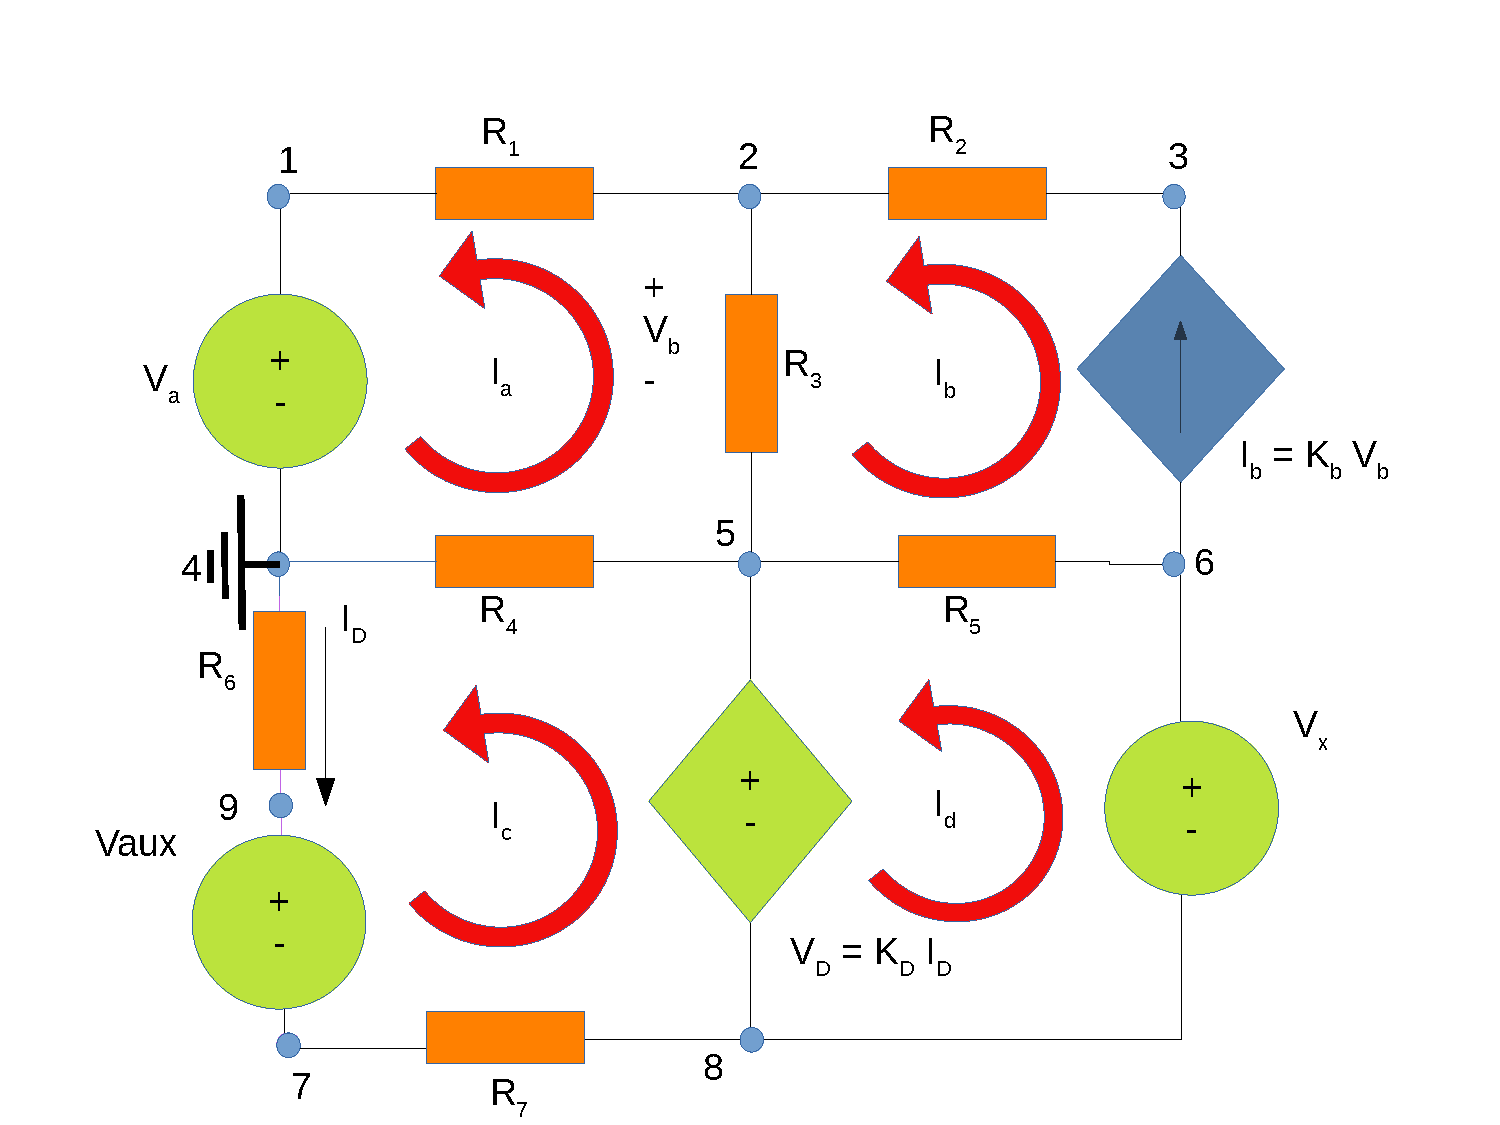
\includegraphics[width=1.0\linewidth]{sim2draw.pdf}
\caption{RC Circuit analysed in section 2.}
\label{sim2draw}
\end{figure}
\par
Then, the values of current of  every branch and the nodal values are obtained using node method. The matrix used in octave is the one that follows.

$\begin{bmatrix}
1 & 0 & 0 & 0 & 0 & 0 & 0 & 0 & 0\\
-G1 & G1+G2+G3 & -G2 & 0 & -G3 & 0 & 0 & 0 & 0\\
0 & -G2-Kb & G2 & 0 & Kb & 0 & 0 & 0 & 0\\
0 & 0 & 0 & 1 & 0 & 0 & 0 & 0 & 0\\
0 & -G1 & 0 & 0 & -G4 & 0 & -G6 & 0 & 0\\
0 & Kb & 0 & 0 & -G5-Kb & G5 & 0 & 0 & 1\\
0 & 0 & 0 & 0 & 0 & 0 & G6+G7& -G7 & 0\\
0 & 0 & 0 & 0 & 0 & 1 & 0 & -1 & 0\\
0 & 0 & 0 & KdG6 & -1 & 0 & -Kd*G6 & 1 & 0
\end{bmatrix}$
$\begin{bmatrix}
V1 \\ V2 \\ V3 \\ V4 \\ V5 \\ V6 \\ V7 \\ I_{x}
\end{bmatrix}$
= 
$\begin{bmatrix}
0 \\ 0 \\ 0 \\ 0 \\ 0 \\ 0 \\ 0 \\ V_{x} \\ 0
\end{bmatrix}$

\par Theoretically speaking, once the voltage source is equal to 0V, $V_{4}$ and  $V_{1}$ are also to be 0. 


\subsection{Operating Point Analysis}
As requested, an operating point analysis was conducted. The capacitor was replaced by the independent voltage source $V_{x}$ (\ref{sim2draw}). The values of currents and nodal voltages  were then put in a table, as well as the $R_{eq}$, hence:

\begin{equation}
R_{eq}=\frac{v(6)-v(8)}{vx#branch}}
\label{eq:4}
\end{equation}


\subsection{Comparison}
After running the node analysis in octave and the simulation in ngspice, the results were put in the tables below. Then, a careful analysis of the aforementioned tables was conducted.

A variable preceded by @ is of type {\em current} and expressed in Ampere; other variables are of type {\it voltage} and expressed in
    Volt. $R_{eq}$ is presented as in \ref{eq:4} in Ohm.

In order to validate the results obtained in NGSPICE, relative errors between the theoretical values, obtained in octave and the ones obtained in ngspice, were calculated. These were put in the table below.

\begin{table}[ht]
\parbox{.30\linewidth}{
  \centering
  \begin{tabular}{|l|r|}
    \hline    
    {\bf Name} & {\bf Value [A or V]} \\ \hline
    @c1[i] & 0.000000e+00\\ \hline
@gb[i] & 0.000000e+00\\ \hline
@r1[i] & 0.000000e+00\\ \hline
@r2[i] & 0.000000e+00\\ \hline
@r3[i] & 0.000000e+00\\ \hline
@r4[i] & 0.000000e+00\\ \hline
@r5[i] & 0.000000e+00\\ \hline
@r6[i] & 0.000000e+00\\ \hline
@r7[i] & 0.000000e+00\\ \hline
v(1) & 0.000000e+00\\ \hline
v(2) & 0.000000e+00\\ \hline
v(3) & 0.000000e+00\\ \hline
v(5) & 0.000000e+00\\ \hline
v(6) & 0.000000e+00\\ \hline
v(7) & 0.000000e+00\\ \hline
v(8) & 0.000000e+00\\ \hline
v(9) & 0.000000e+00\\ \hline

  \end{tabular}
  \caption{Simulation and Calculus of Req (NgSpice)}} 
\parbox{.30\linewidth}{
  \centering
  \begin{tabular}{|l|r|}
    \hline    
    {\bf Name} & {\bf Value [A or V]} \\ \hline
    V1 & 0.000000e+00 \\ \hline
V2 & 0.000000e+00 \\ \hline
V3 & 9.496396e-16 \\ \hline
V4 & 0.000000e+00 \\ \hline
V5 & 5.935248e-17 \\ \hline
V6 & 8.553593e+00 \\ \hline
V7 & -2.967624e-17 \\ \hline
V8 & 0.000000e+00 \\ \hline
Ix & -2.745419e-03 \\ \hline
Req & 3.115588e+03 \\ \hline
tau & 3.244185e-03 \\ \hline

  \end{tabular}
  \caption{Calculus of R_{eq}- Octave}}
 
\end{table}

\par After the careful evaluation of the results, several observations need to be made. Firstly, in ngspice, there are some node voltage results different from 0V, with  values  in the order of magnitude of 10^-15, 10^-16 V. After questioning the professor, these will be considered 0V.

\par On the other hand, octave results have equally those discrepancies. That said, the procedure was the same and those values were considered 0. We believe the main reason for this situation is that, when the data.txt file is read from the datagen.py in octave, a rounding happens, making it impossible for the nodal voltages to be 0. 

\par However, and despite the small erros above explaned, the values of $R_{eq}$, $V_{6}$ and $I_{x}$ match perfectly, which led us to fully validate the theorical procedure and the results obtained.




 

